最後に$\varphi$が全単射であることを証明する.そのために次の概念を導入する.

\begin{defin}
  path $p_1,\cdots,p_k$を$1$辺の長さが$n+k$の正三角形に図\ref{generic puzzle}のように配置したとき,重なってしまうpieceが存在する場合,このpuzzle $P$はskew puzzleであると呼ぶ.
\end{defin}

skew puzzleに対しても$\varphi$によってedge labeled tableauxを対応させることができるが,次の補題が成り立つ.

\begin{lemm}\label{skew puzzle}
  $P$がskew puzzleであることと$\text{EqRect}(\varphi(P))\neq T_{\mu}$であることは同値である.
\end{lemm}

\begin{proof}
  命題\ref{main theorem 1}より,$\text{EqRect}(\varphi(P))\neq T_{\mu}$ならば$P$はskewではない.

  
\end{proof}

\begin{prop}
  $\varphi\colon\mathcal{P}^\nu_{\lambda\mu}\rightarrow\mathcal{T}^\nu_{\lambda\mu}$は全単射である.
\end{prop}

\begin{proof}
  $T\in \mathcal{T}^\nu_{\lambda\mu}$に対して,path $p_1,\cdots,p_k$をつぎのように定める.

  まず$p_k$のsegment $s_{k,1}$を決定する.piece 
  
\begin{tikzpicture}[baseline=-1pt]
    \fill[cyan] (0,0)--(0.25,0.42)--(0.5,0)--(0.25,-0.42)--cycle;
    \draw[thick] (0,0)--(0.25,0.42)--(0.5,0)--(0.25,-0.42)--cycle;
  \end{tikzpicture}
  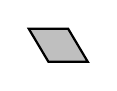
\begin{tikzpicture}[baseline=2pt]
    \fill[lightgray] (0,0)-- ++(0.5,0)-- ++(-0.25,0.42)-- ++(-0.5,0)--cycle;
    \draw[thick](0,0)-- ++(0.5,0)-- ++(-0.25,0.42)-- ++(-0.5,0)--cycle;
  \end{tikzpicture}
  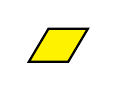
\begin{tikzpicture}[baseline=2pt]
    \fill[yellow] (0,0)-- ++(0.5,0)-- ++(0.25,0.42)-- ++(-0.5,0)--cycle;
    \draw[thick](0,0)-- ++(0.5,0)-- ++(0.25,0.42)-- ++(-0.5,0)--cycle;
  \end{tikzpicture}
  それぞれ文字 $text{b},\text{g},\text{y}$と同一視し,segment に含まれるpiece を上から読んで,$text{b},\text{g},\text{y}$からなる文字列と同一視する.

  $T$の$k$行目の最も右にある箱を$x$とおく.$\alpha = |\mu|$,$s_{k,1}$は空の文字列とする.
  \[
  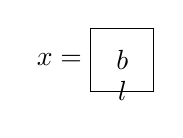
\begin{tikzpicture}
    \node at (-0.4, -0.4) {$x=$};
    \draw (0,0) rectangle ++(0.8,-0.8);
    \node at (0.4,-0.4) {$b$};
    \node at (0.4,-0.8) {$l$};
  \end{tikzpicture}
  \]
  としたとき,$\alpha = b$ならば$s_{k,1}$の左に$\text{y}$を付け足す.$\alpha\in l$ならば$s_{k,1}$の左に$\text{b}$を付け足す.$\alpha\neq b$かつ$\alpha\notin l$ならば$s_{k,1}$の左に$\text{g}$を付け足す.$x$の左に箱が存在するならば$x$を$x$の左の箱に置き換え,$\alpha$を$\alpha -1$に置き換えて同じ操作をする.$x$の左に箱が存在しないならば操作を終了する.

  次に$s_{k-1,2}$を決定する.$\alpha$は$s_{k,1}$に対する操作が終了したときと同じまま,$x$は$T$の$k-1$行目の最も右にある箱とする.


  
  補題\ref{skew puzzle}より$p_1,\cdots,p_k$はpuzzle $P$を定め,$\varphi(P)=T$である.

  $\varphi(P)=\varphi(P')$であるならば,$P$と$P'$に含まれるpathは等しいから,$P=P'$でなければならない.
\end{proof}